\section{Доказательство непланарности графов $K_5$ и $K_{3,3}$. Критерий планарности графов. Выяснить, 
является ли граф планарным.}

С помощью следствия из теоремы Эйлера можно доказать непланарность
некоторых графов.

Рассмотрим полный граф $K_5$. У него $n=5, r=10$.
\begin{figure}[h]
    \centering
    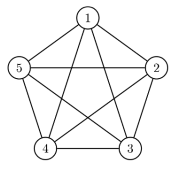
\includegraphics[scale=0.4]{32_1.png}
\end{figure}

$3 \cdot 5 - 10 = 5 < 6$, поэтому этот граф не является планарным.

Рассмотрим полный двудольный граф $K_{3,3}$.
\begin{figure}[h]
    \centering
    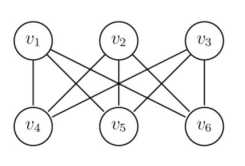
\includegraphics[scale=0.4]{32_2.png}
\end{figure}

У него $n=6, r = 9$. Если бы граф $K_{3,3}$ был планарным, то из равенства
$6 - 9 + q = 2$ получаем: $q=5$, поэтому $5 = q_3 + q_4 + \dots$

У графа K3,3 циклы минимальной длины могут иметь длину 4, циклов длины
5 нет (у двудольного графа циклы не могут иметь нечетную длину), могутеще быть циклы длины 6,
поэтому $5 = q_4 + q_6$ Решениями этого уравнения
являются пары: (0,5), (1,4), (2,3), (3,2), (4,1), (5,0).

Имеем также равенство: $2r = 18 = 4q_4 + 6q_6$. Ни одна из пар предыдущего
равенства не является решением этого уравнения.

Поэтому граф $K_{3,3}$ не является планарным.

Граф $K_{3,3}$ связан с теоремой о трех соседях и трех колодцах: нужно от
каждого из домов трех соседей к каждому из трех колодцев провести
дорожки, которые бы не пересекались. Так как граф $K_{3,3}$ не является
планарным, то это сделать невозможно.

\begin{theorem}
    \textbf{(Критерий Понтрягина -- Куратовского плоской реализуемости
графа)}

    Конечный граф $G$ является планарным тогда и только тогда, когда он не имеет
    подграфов, гомеоморфных $K_5$ или $K_{3,3}$.
\end{theorem}